\chapter{Lecture 9: New Revolutions in Particle Physics: Standard Model}

These companion notes follow Leonard Susskind's ninth lecture in the supplementary \emph{Particle Physics 2 Standard Model} course, with curation by LazyingArt LLC. The lecture begins by rewinding to a deliberately simplified \(U(1)\) model, not because the Standard Model is actually so simple, but because in that toy setting one can see the Higgs mechanism unfold line by line. From there the argument turns to fermions and makes the same point again in a sharper form: masses are not freely inserted where symmetry forbids them; they appear only after the Higgs field settles into a symmetry-breaking vacuum.

\section{Gauge-Field Recap and the Meaning of Masslessness}

Susskind begins by going back to the gauge field itself. The board-level reminder is the field-strength tensor together with the shorthand \(F^2\), which in the lecture stands for the gauge-field kinetic term.

\begin{figure}[t]
\centering

\includegraphics[width=0.72\textwidth]{lecture_09_figure_02.png}
\caption{Field-strength definition and \(F^2\) shorthand.}
\end{figure}

We rewrite the board equation in standard indexed form:
\begin{equation}
F_{\mu\nu}=\partial_\mu A_\nu-\partial_\nu A_\mu.
\end{equation}
The gauge-field Lagrangian is then of the schematic form
\begin{equation}
\mathcal{L}_{\mathrm{gauge}} \propto F_{\mu\nu}F^{\mu\nu},
\end{equation}
with the overall normalization suppressed, just as it is in the lecture.

The key point is not the normalization but the derivatives. Since \(F_{\mu\nu}\) contains only derivatives of \(A_\mu\), a homogeneous shift
\begin{equation}
A_\mu(x)\longrightarrow A_\mu(x)+c_\mu,
\qquad \partial_\nu c_\mu=0,
\end{equation}
leaves \(F_{\mu\nu}\) unchanged. In the field-theoretic sense used throughout the lecture, that means there is no energy cost for shifting the gauge field uniformly everywhere. A zero-momentum excitation therefore carries no rest energy, and the gauge boson is massless.

\begin{remark}
Throughout this chapter the mathematics is written in a toy \(U(1)\) language. Whenever the lecture speaks loosely of a ``photon mass,'' the intended physical application is the analogous mass generation for the \(W\) and \(Z\), not a literal mass for the QED photon.
\end{remark}

\section{Broken Higgs Field and Gauge-Boson Mass}

Now the lecture adds the new ingredient: a charged Higgs field. It is written in polar form as
\begin{equation}
\phi=\rho e^{i\alpha}.
\end{equation}
The potential energy is assumed to have the Mexican-hat form, so that the minimum is not at \(\phi=0\) but at a nonzero radius. On the board this vacuum value is written as lower-case \(f\); in the notes we will use upper-case \(F\) for the same quantity.

\begin{figure}[t]
\centering

\includegraphics[width=0.72\textwidth]{lecture_09_figure_03.png}
\caption{Frozen Higgs field and broken-phase covariant derivative.}
\end{figure}

The lecture then makes the first approximation that drives the whole calculation: the radial direction is stiff, so we freeze it and allow only the phase to vary,
\begin{equation}
\phi(x)\approx F e^{i\alpha(x)}.
\end{equation}
The faint sketch on the board is only a reminder of that radial slice through the potential; the real content is simply that the minimum occurs at nonzero \(F\) and that radial motion is costly.

\begin{figure}[t]
\centering
\begin{tikzpicture}[scale=1.0]
\draw[->] (0,0) -- (5.4,0) node[right] {$\rho$};
\draw[->] (0,0) -- (0,3.3) node[above] {$V(\rho)$};
\draw (0.15,2.6) .. controls (0.75,2.0) and (1.25,1.0) .. (2.05,0.82)
      .. controls (2.55,0.75) and (3.10,1.20) .. (4.70,2.75);
\draw[dashed] (2.05,0) -- (2.05,0.82);
\fill (2.05,0.82) circle (1.4pt);
\node[below] at (2.05,0) {$F$};
\end{tikzpicture}
\caption{A clean radial slice of the broken Higgs potential. The lecture uses only the nonzero minimum and the stiffness of the radial direction.}
\end{figure}

\paragraph{Worked derivation.}
At this point Susskind computes the covariant derivative in the frozen-radius approximation. The lecture is unstable about the sign, and he says so explicitly, so we choose one consistent convention,
\begin{equation}
D_\mu=\partial_\mu+iA_\mu,
\end{equation}
with the gauge coupling suppressed. Then
\begin{align}
\phi(x)&\approx F e^{i\alpha(x)},\\
D_\mu\phi
&=(\partial_\mu+iA_\mu)\bigl(F e^{i\alpha}\bigr),\\
&\approx i\bigl(\partial_\mu\alpha+A_\mu\bigr)F e^{i\alpha}.
\end{align}
Squaring the covariant derivative gives the piece of the Higgs Lagrangian that matters here:
\begin{equation}
|D_\mu\phi|^2 \approx F^2\bigl(\partial_\mu\alpha+A_\mu\bigr)\bigl(\partial^\mu\alpha+A^\mu\bigr).
\end{equation}
The decisive observation now follows the lecture exactly: the combination \(A_\mu+\partial_\mu\alpha\) is itself just a gauge-transformed vector potential. Define
\begin{equation}
A'_\mu=A_\mu+\partial_\mu\alpha.
\end{equation}
Then the same term becomes
\begin{equation}
|D_\mu\phi|^2 \approx F^2 A'_\mu A'^\mu.
\end{equation}

\begin{figure}[t]
\centering

\includegraphics[width=0.72\textwidth]{lecture_09_figure_04.png}
\caption{Emergent \(f^2A^2\) term in the broken phase.}
\end{figure}

This is the first climax of the lecture. The phase field \(\alpha\) has disappeared into the redefined gauge potential \(A'_\mu\), and what survives is a no-derivative quadratic term for the gauge field. In the language of the lecture, the Goldstone boson has been eaten, while the radial excitation that we froze out remains available as a massive Higgs mode if the system is excited hard enough.

\subsection{Question \& Answer}

Why does an \(A'^2\) term mean mass?

The lecture answers this by stepping back from the formula. In relativity, mass is the energy of the system at rest. In field theory, a particle at rest corresponds to a mode of zero momentum, hence infinite wavelength, hence a homogeneous shift of the field. So the question is really this: if we shift the field uniformly everywhere, does the energy change?

For the original gauge-field term the answer was no, because only derivatives appeared. A uniform shift left the field strength untouched. But once the broken Higgs phase produces
\begin{equation}
F^2 A'_\mu A'^\mu,
\end{equation}
a homogeneous shift
\begin{equation}
A'_\mu(x)\longrightarrow A'_\mu(x)+c_\mu
\end{equation}
does change the energy:
\begin{equation}
\Delta \mathcal{E}\propto F^2 c_\mu c^\mu.
\end{equation}
That nonzero stored energy at zero momentum is precisely what the lecture calls the mass of the gauge boson.

Susskind then slows the discussion further with analogies. A long-wavelength phonon in a crystal is massless because shifting the whole lattice rigidly costs no energy. A spin wave in a magnet is massless for the same reason: rotate all the little magnets together and nothing resists. But if positive and negative charges in a medium are shifted against one another, even homogeneously, there is a restoring force and the mode becomes massive; that is the plasmon analogy. The Higgs mechanism is being put in this same class. What used to be a derivative-only, Goldstone-like mode has coupled to the gauge field in such a way that a uniform displacement now costs energy.

\section{Weak Interactions, Handedness, and the Chiral Asymmetry of Nature}

Only after the gauge-boson story is secure does the lecture turn to fermions. The opening move is experimental, not algebraic. Weak interactions violate left-right reflection symmetry. In quantum electrodynamics and quantum chromodynamics, mirror-reflected processes are equally allowed; in the weak interactions, left and right are treated differently.

In the lecture's deliberately loose language, a fast particle is called right-handed if its spin is along its momentum and left-handed if its spin is opposite to its momentum. With that understood, the empirical weak-interaction rule is
\begin{equation}
W:\qquad e_L \leftrightarrow \nu_L,
\qquad e_R \ \text{does not couple in this simplified discussion.}
\end{equation}
Likewise, beta decay produces the left-handed electron and not the right-handed one. The same asymmetry extends beyond that one process: the weak interaction singles out the left-handed electron and the left-handed neutrino.

\begin{remark}
The lecture is explicit that this discussion is loose about helicity versus chirality. For highly energetic particles the distinction is less dangerous, and that is the regime Susskind uses to motivate the physics. Later notes can sharpen the terminology; here the priority is to preserve the lecture's logic.
\end{remark}

This empirical fact creates the next obstruction. If left and right are not on equal footing under the weak symmetry, then a fermion mass cannot simply be assumed; one must explain how the left-handed and right-handed components can possibly talk to each other.

\section{Dirac Mass as Left-Right Mixing, and Why the Weak Symmetry Blocks It}

Susskind now goes back to the Dirac equation for the same reason he went back to \(F_{\mu\nu}\) earlier: he wants the meaning of the mass term to be read directly from the equation.

\begin{figure}[t]
\centering

\includegraphics[width=0.74\textwidth]{lecture_09_figure_05.png}
\caption{Coupled left- and right-handed fermion equations.}
\end{figure}

In the board notation, the massless Dirac equation is written schematically as
\begin{equation}
i\left(\frac{\partial \Psi}{\partial t}+\alpha_i\frac{\partial \Psi}{\partial x_i}\right)=0.
\end{equation}
Again the important point is that only derivatives appear. By the same logic used for the gauge field, that means there is no rest-energy cost for a homogeneous shift of the field, and the fermion is massless.

To add mass, the lecture restores the fourth Dirac matrix \(\beta\):
\begin{equation}
i\left(\frac{\partial \Psi}{\partial t}+\alpha_i\frac{\partial \Psi}{\partial x_i}\right)=m\beta\Psi.
\end{equation}
The board version of the split equations is not notation-stable, and Susskind later admits that some factors of \(i\) were handled inconsistently. A cleaned version that preserves the lecture's structural point is
\begin{align}
i\left(\frac{\partial \Psi_R}{\partial t}+ i\,\alpha_i\frac{\partial \Psi_R}{\partial x_i}\right)&=m\Psi_L,\\
i\left(\frac{\partial \Psi_L}{\partial t}- i\,\alpha_i\frac{\partial \Psi_L}{\partial x_i}\right)&=m\Psi_R.
\end{align}
These equations say exactly what the lecture wants them to say: the mass term couples left-handed and right-handed components. If \(m=0\), the two sectors decouple. If \(m\neq 0\), left turns into right and right turns into left.

Now comes the fake world that sharpens the obstruction. Suppose, as a toy model of the weak interaction, that only the left-handed fermion carries the relevant \(U(1)\) charge. Then
\begin{equation}
\Psi_L \longrightarrow e^{i\theta}\Psi_L,
\qquad
\Psi_R \longrightarrow \Psi_R.
\end{equation}
The derivative terms on the left-hand sides transform the same way as the fields themselves, but the mass terms do not match between left and right. In one equation the right-hand side picks up a phase while the left-hand side does not, and in the other equation the mismatch goes the other way. Therefore the bare mass term is not symmetry-invariant in this toy weak-asymmetric world.

This is the second major tension of the lecture. If weak interactions really distinguish left from right, how can the electron, the muon, the quarks, or anything like them ever become massive?

\subsection{Question \& Answer}

If left and right transform differently, how can fermions get mass?

The answer is to introduce another charged field and to let the would-be mass term borrow its charge from that field. Let \(\phi\) be a bosonic field with transformation rule
\begin{equation}
\phi\longrightarrow e^{i\theta}\phi,
\qquad
\phi^*\longrightarrow e^{-i\theta}\phi^*.
\end{equation}
Then instead of the forbidden bare mass term, we write the symmetry-respecting Yukawa coupling:
\begin{align}
i\left(\frac{\partial \Psi_R}{\partial t}+ i\,\alpha_i\frac{\partial \Psi_R}{\partial x_i}\right)&=g\,\phi^*\,\Psi_L,\\
i\left(\frac{\partial \Psi_L}{\partial t}- i\,\alpha_i\frac{\partial \Psi_L}{\partial x_i}\right)&=g\,\phi\,\Psi_R.
\end{align}
Now the phases cancel correctly. In the first equation \(\phi^*\) cancels the phase of \(\Psi_L\); in the second, \(\phi\) carries exactly the phase that \(\Psi_L\) carries. So the symmetry survives.

This is the lecture's ``trick.'' Left-right conversion is now allowed, but not for free. It can only happen together with the charged scalar field, and the strength of the process is governed by the new constant \(g\), the Yukawa coupling.

\begin{figure}[t]
\centering
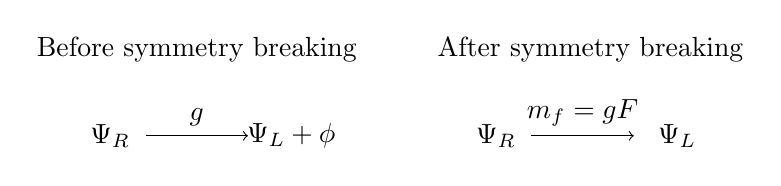
\begin{tikzpicture}[x=1cm,y=1cm]
\node at (2.0,2.1) {Before symmetry breaking};
\node at (7.0,2.1) {After symmetry breaking};
\node at (0.9,1.0) {$\Psi_R$};
\node at (3.2,1.0) {$\Psi_L+\phi$};
\draw[->] (1.35,1.0) -- (2.65,1.0) node[midway,above] {$g$};
\node at (5.8,1.0) {$\Psi_R$};
\node at (8.1,1.0) {$\Psi_L$};
\draw[->] (6.25,1.0) -- (7.55,1.0) node[midway,above] {$m_f=gF$};
\end{tikzpicture}
\caption{The Yukawa mechanism in schematic form. Before symmetry breaking, left-right conversion is accompanied by the charged scalar; after \(\phi\) is replaced by its vacuum value, the same coupling becomes an effective fermion mass.}
\end{figure}

\section{Yukawa Masses, Neutrinos, and the Final Unification Around \(F\)}

Now the lecture returns to the Higgs field. Suppose that the scalar \(\phi\) is precisely the Higgs field we have already discussed, so that in the broken phase its magnitude is approximately frozen at the nonzero value \(F\). Then the Yukawa term becomes
\begin{equation}
g\phi \approx gF,
\qquad
g\phi^* \approx gF,
\end{equation}
and the effective fermion mass is simply
\begin{equation}
m_f=gF.
\end{equation}
This is the fermionic version of the same mechanism that gave the gauge boson a mass. In the gauge sector, the shift of the Higgs field produced a term proportional to \(F^2 A_\mu A^\mu\). In the fermion sector, the same shift produces the left-right mixing coefficient \(m_f\).

But the Higgs field is not really frozen forever. The lecture insists on that point too. If we restore the radial excitation \(h\), then schematically
\begin{equation}
\phi \approx F+h,
\end{equation}
so the same Yukawa term becomes
\begin{equation}
g\phi \approx gF + gh.
\end{equation}
The first piece is the fermion mass; the second is the coupling of the physical Higgs boson to that fermion. At the lecture's 2010 horizon, this is already presented as an experimental program: once Higgs production and decay are observed, one should check whether the relative rates track the same Yukawa couplings that account for the fermion masses.

The hierarchy of fermion masses is therefore pushed into a hierarchy of Yukawa couplings. Susskind estimates, at the order-of-magnitude level of the lecture, that
\begin{equation}
g_e \sim \frac{m_e}{\text{weak scale}} \sim \frac{0.5\,\mathrm{MeV}}{10^2\,\mathrm{GeV}} \sim 10^{-5},
\end{equation}
while for the top quark one finds a coupling of order one,
\begin{equation}
g_t=\mathcal{O}(1).
\end{equation}
The Standard Model does not explain this spectrum; it parameterizes it.

The lecture then turns, more cautiously, to neutrinos. In the simplest Standard Model presentation, neutrinos are left-handed and were once taken to be massless. But the lecture already takes seriously the fact that neutrino oscillations imply tiny nonzero masses. The key formal point remains the same: for fermions, mass means left-right mixing. For a neutrino, however, the right-handed state that mixes with \(\nu_L\) may be the right-handed antineutrino:
\begin{equation}
\nu_L \longleftrightarrow \bar{\nu}_R.
\end{equation}
That possibility is unavailable for the electron because the electron cannot mix with its antiparticle without violating electric charge conservation. The neutrino is different, and that is what leads the lecture to the Majorana idea: a fermion whose mass arises by mixing the particle with its own antiparticle.

The final synthesis is broad but clear. In this simplified presentation, the known Standard Model masses all trace back to the same symmetry-breaking scale \(F\). The gauge bosons are massless before the shift because gauge symmetry forbids a bare mass. The fermions are massless before the shift because their left-handed and right-handed pieces transform differently under the weak symmetry, so a direct mass term is forbidden there as well. After the Higgs field moves away from the symmetric vacuum, both obstacles are bypassed.

\section{Summary}

The lecture does two things in parallel. First, it re-derives the Higgs mechanism for gauge bosons in the cleanest possible toy setting: freeze the Higgs radius, keep the phase, compute \(D_\mu\phi\), and discover that the Goldstone mode is absorbed into the gauge field, leaving behind an \(A_\mu A^\mu\)-type mass term. Second, it repeats the same logic for fermions: a fermion mass is left-right mixing, but that mixing is forbidden if left and right transform differently under the weak symmetry, so the Higgs field must enter through a Yukawa coupling and only afterward reduce to \(m_f=gF\).

That is the lecture's central unification. In this simplified \(U(1)\) narrative, the masses of the \(W\) and \(Z\), the masses of the charged leptons and quarks, and even the suggestive neutrino story all point back to one symmetry-breaking scale. The details are species-dependent, but the source is shared: without the Higgs field sitting at nonzero \(F\), the familiar particles would remain massless.